\documentclass[10pt,a4paper]{article}

%--- packages --------------------------------------------------------
\usepackage[margin=2.5cm]{geometry}
\usepackage{amsmath,amssymb}
\usepackage{graphicx}
\usepackage{booktabs}
\usepackage[hidelinks]{hyperref}          % remove colored link boxes
\usepackage{natbib}
\usepackage{caption}
\usepackage{subcaption}
\usepackage{microtype}
\usepackage{setspace}
\usepackage[table]{xcolor}                % table row coloring
\onehalfspacing

%--- caption formatting -----------------------------------------------
\captionsetup{font=small, labelfont=bf}

%--- metadata --------------------------------------------------------
\title{\Large\textbf{Gene-Selection Optimization via JTK\_Cycle Pre-Filtering:}\\
       \Large\textbf{Reproducing and Extending \emph{TimeSignature}}}

\author{
  \normalsize Nahye Kim\textsuperscript{1} \quad
  Jaehyeon Lee\textsuperscript{2}\\
  {\small \textsuperscript{1}Electrical Engineering, KAIST \quad
   \textsuperscript{2}School of Computing, KAIST}\\[8pt]
}

\date{}

%=====================================================================
\begin{document}
\maketitle

\vspace{0.5em}
\noindent\rule{\linewidth}{0.4pt}
\vspace{-4pt}

\noindent{\small \textbf{Code Availability:} The complete R source code, including the implementation of the JTK\_Cycle pre-filtering pipeline and simulation scripts, is openly available on GitHub at 
\url{https://github.com/jaedungg/BCS40010_TimeSignature-ext}.}

\vspace{4pt}
\noindent\rule{\linewidth}{0.4pt}
\vspace{1.5em}

%=====================================================================
\begin{abstract}
%=====================================================================
Circadian-time prediction from blood transcriptomes has direct
clinical applications in chronotherapy and circadian phenotyping.
\emph{TimeSignature} addresses this prediction task by training an
elastic-net regression over all ${\sim}$7,600 genes in a microarray
panel and recovering ${\sim}$40 predictors without any prior
periodicity screen.
This unfiltered training scheme leaves most of the candidate pool
non-rhythmic, raising the question of whether a periodicity screen
could yield an equally accurate but far smaller predictor set.
Such a screen is exactly what subsequent methods---\emph{TimeMachine}
and \emph{tauFisher}---introduce, inserting a JTK\_Cycle rhythmicity
pre-filter before regression to reduce the candidate pool to
20--37 genes.
Whether this same pre-filtering strategy can improve TimeSignature's
gene-selection efficiency, yielding a smaller predictor set that still
meets clinically acceptable accuracy (nAUC $\geq 0.80$,
MAE $< 2.5$\,h) under the original two-blood-draw protocol, is the
question we address here.
To answer this question, two experiments are conducted on four public datasets
(GSE39445, GSE48113, GSE56931, GSE113883).
Experiment~1 sweeps the elastic-net candidate pool from 10 to
7,615 genes ordered by JTK\_Cycle rhythmicity rank, producing a
gene-count versus accuracy trade-off curve.
Experiment~2 substitutes five published or derived gene
sets---including the TimeSignature core-18, TimeMachine-37,
tauFisher, canonical core-clock genes, and their
intersection---directly into the TimeSignature framework.
Across these experiments, a JTK-filtered pool of only 30 genes achieves
nAUC\,${=}\,0.833$ and MAE\,${=}\,2.13$\,h, within 0.020 nAUC of
the full-panel model while screening fewer than 0.4\% of the
transcriptome.
Among published gene sets, a panel reconstructed following the
TimeMachine procedure performs best
(nAUC\,${=}\,0.844$), whereas canonical clock genes alone fall below
the clinical floor (nAUC\,${=}\,0.792$), indicating that the
circadian prediction signal resides in data-driven rhythmic genes
rather than the textbook feedback loop.
\end{abstract}

%=====================================================================
\section{Introduction}
%=====================================================================

The circadian clock governs nearly every aspect of human physiology,
from hormone secretion and immune function to drug metabolism and cell
division \citep{Reppert2002}.
This pervasive regulation is reflected at the molecular level by
widespread 24-hour rhythms in gene expression across human tissues
\citep{Talamanca2023}.
Such rhythms make the precise estimation of an
individual's internal circadian phase---often termed the
\emph{circadian time}---a prerequisite for personalized chronotherapy,
shift-work assessment, and circadian disorder diagnosis
\citep{Archer2014}.
The gold-standard measure of circadian phase is the dim-light
melatonin onset (DLMO), which requires controlled light conditions
and repeated nocturnal sampling.
These stringent requirements make DLMO impractical in routine clinical
settings, motivating the search for biomarker-based alternatives
\citep{Ueda2004}.
Blood transcriptomics offers one such alternative: circadian gene
expression in peripheral blood tracks internal time with sufficient
precision for clinical use \citep{Moller2013}, and single-sample
assays such as BodyTime have shown that a compact panel of blood
transcripts can estimate internal circadian time with accuracy
comparable to DLMO \citep{Wittenbrink2018}.

Building on this observation, Braun et al.\ (2018) introduced
\emph{TimeSignature}, an elastic-net model that predicts local
sampling time from whole-blood microarray profiles \citep{Braun2018}.
TimeSignature requires two blood draws approximately 12\,h apart for
within-subject normalization;
it trains on all ${\sim}$7,600 genes in
the cross-study intersection and lets the elastic-net penalty
implicitly select ${\sim}$40 predictors.
This approach achieves a normalized AUC (nAUC) of ${\sim}$0.85 and a
median absolute error below 2\,h on four independent datasets.
Despite this strong cross-study performance, the method enters the
elastic net with no prior periodicity screen, so the majority of the
${\sim}$7,600-gene pool carries no circadian signal and may add noise
to the covariate matrix.

Later methods addressed this inefficiency by pre-filtering genes with
JTK\_Cycle \citep{Hughes2010}, a non-parametric rank-correlation test
that identifies 24-hour rhythms in time-series expression data;
related algorithms have since been developed to disclose oscillations
in transcription with improved sensitivity \citep{Antoulas2018}.
TimeMachine (Huang \& Braun, 2024) applies JTK\_Cycle to reduce
the candidate pool to 37 rhythmic genes before fitting a penalized
regression for single-sample circadian-time estimation
\citep{Huang2024}.
tauFisher (Duan \& Ngo, 2024) likewise anchors its predictor on
canonical core-clock genes augmented by JTK\_Cycle-ranked rhythmic
genes \citep{Duan2024}.
Both studies demonstrate that pre-filtering can produce compact,
interpretable gene panels, but neither quantifies the \emph{trade-off}
between pool size and prediction quality within the original
two-draw TimeSignature framework.

The present work fills this gap.
We first reproduce the TimeSignature Figure~1 benchmark and then
systematically explore how JTK\_Cycle pre-filtering affects
gene-selection efficiency.
Two experiments quantify the gene-count versus accuracy trade-off:
Experiment~1 sweeps the JTK-filtered pool size from 10 to the full
7,615 genes, and Experiment~2 substitutes five published gene sets
into the same pipeline.
These experiments together identify the minimum rhythmic gene set
that preserves clinically acceptable accuracy (nAUC $\geq 0.80$,
MAE $< 2.5$\,h) under the two-blood-draw protocol of the original
study.

%=====================================================================
\section{Methods}
%=====================================================================
 
\subsection{Datasets}
 
All experiments use the four datasets bundled with the public
TimeSignatR package (Table~\ref{tab:datasets}).
The GSE39445 training half (subjects assigned \texttt{train\,=\,1})
provides ${\sim}$213 samples from the Möller-Levet sleep-restriction
study; these samples serve exclusively for model training and
JTK\_Cycle ranking.
The remaining three studies constitute held-out validation sets:
GSE48113 (Archer et al.; $n = 286$), GSE56931 (Arnardottir et al.;
$n = 249$), and GSE113883 (RNA-seq; $n = 153$).
Across all four studies, 7,615 genes are present on every platform;
this common intersection defines the full gene universe.
 
\begin{table}[h]
\centering
\caption{Datasets used in this study.  All four share a common
set of 7,615 genes.}
\label{tab:datasets}
\begin{tabular}{lllrl}
\toprule
GEO accession & Study & Role & $n$ & Platform \\
\midrule
GSE39445  & Möller-Levet et al.\ (2013) & Training      & ${\sim}$213 & Microarray \\
GSE48113  & Archer et al.\ (2014)       & Validation (V1) & 286 & Microarray \\
GSE56931  & Arnardottir et al.\ (2014)  & Validation (V2) & 249 & Microarray \\
GSE113883 & ---                          & Validation (V3) & 153 & RNA-seq \\
\bottomrule
\end{tabular}
\end{table}
 
\subsection{Baseline Pipeline (Braun et al., 2018)}
 
We briefly summarise the three components of the original
TimeSignature pipeline that our extension re-uses unchanged; full
details are given in \citet{Braun2018}.
 
\paragraph{Within-subject normalization.}
Between-subject baseline differences are removed by subtracting, for
each subject, the mean expression vector across that subject's time
points from every individual sample.
The resulting genes $\times$ samples matrix (\texttt{trainWSN}) is
used for both JTK\_Cycle ranking and elastic-net training.
 
\paragraph{Circular elastic-net regression.}
Sampling time $t$ is encoded as unit-circle coordinates
$\mathbf{y} = (\sin 2\pi t/24,\allowbreak \cos 2\pi t/24)$, and a
multivariate Gaussian elastic net
(\texttt{family\,=\,"mgaussian"}, $\alpha = 0.5$) is fit with
\texttt{cv.glmnet}; the penalty $\lambda$ is selected at
\texttt{lambda.min}.
Predicted time is recovered by
$\hat t = (24/2\pi)\,\mathrm{atan2}(\hat y_1,\hat y_2) \bmod 24$.
The only modification in our extension is which rows (genes) of the
expression matrix are passed to this regression---the regression
itself is unchanged.
 
\paragraph{Antipodal calibration (two-blood-draw protocol).}
At test time, each subject provides two blood samples
${\sim}$12\,h apart; each sample is centred on the mean of the pair
($\mathbf{x}_s^{\mathrm{cal}} = \mathbf{x}_s -
\tfrac{1}{2}(\mathbf{x}_s + \mathbf{x}_{s'})$).
This calibration matrix is computed once across all samples before
any experiment, because it depends only on sample pairing and is
independent of the gene pool.
 
All runs use \texttt{RNGversion("3.5.1")} and
\texttt{set.seed(194)} for exact reproducibility.
 
\subsection{JTK\_Cycle Rhythmicity Ranking}
 
JTK\_Cycle \citep{Hughes2010} tests whether a gene's temporal
expression profile is significantly rhythmic by comparing it, via
Kendall's rank correlation $\tau$, against a family of cosine
reference templates of fixed period $T = 24$\,h.
Our compact re-implementation (\texttt{JTKfns.R}) proceeds in four
steps.
 
\paragraph{Step 1: time-bin aggregation.}
Training samples are partitioned into 1-h circadian-time bins
(modulo 24\,h), and the mean expression of each gene within each
occupied bin is computed.
The result is a bins $\times$ genes matrix $\mathbf{B}$ representing
each gene's aggregated circadian profile.
 
\paragraph{Step 2: Kendall S computation.}
Let $n_b$ denote the number of occupied bins and let
$\mathcal{P} = \binom{n_b}{2}$ be the set of all ordered bin pairs.
For each gene $g$ and each pair $(i,j) \in \mathcal{P}$, define
$\delta_{gij} = \mathrm{sign}(B_{ig} - B_{jg})$.
Similarly, for each of the $M = 24$ equispaced cosine phase
templates
$r^{(k)}(t) = \cos\!\bigl(2\pi(t - \phi_k)/24\bigr)$,
$\phi_k = k$\,h, $k = 0,\ldots,23$, define
$\rho_{ij}^{(k)} = \mathrm{sign}\!\bigl(r^{(k)}(t_i) -
r^{(k)}(t_j)\bigr)$.
The Kendall S statistic at phase template $k$ for gene $g$ is then
\begin{equation}
  S_g^{(k)} = \sum_{(i,j)\in\mathcal{P}}
               \delta_{gij}\,\rho_{ij}^{(k)}.
  \label{eq:kendallS}
\end{equation}
All $S_g^{(k)}$ values are computed simultaneously via the matrix
product $\mathbf{S} = \boldsymbol{\Delta}^\top \mathbf{R}$, where
$\boldsymbol{\Delta}$ is the $|\mathcal{P}| \times G$ gene-sign
matrix and $\mathbf{R}$ is the $|\mathcal{P}| \times M$ template-sign
matrix.
 
\paragraph{Step 3: optimal phase and $\tau$.}
For each gene $g$, the optimal phase template is
$k^* = \arg\max_k |S_g^{(k)}|$.
The Kendall $\tau$ at this optimum is
\begin{equation}
  \tau_g = \frac{S_g^{(k^*)}}{\binom{n_b}{2}},
  \label{eq:tau}
\end{equation}
and the estimated peak phase is $\hat\phi_g = \phi_{k^*}$
(shifted by 12\,h when $S_g^{(k^*)} < 0$ to report the time of
peak).
 
\paragraph{Step 4: p-values.}
Under the null hypothesis of no rhythm, $S$ is approximately normal
with mean 0 and variance $|\mathcal{P}|(2n_b+5)/9$.
The two-sided p-value for the optimal phase is
$p_g = 2\,\Phi(-|S_g^{(k^*)}|/\sigma)$.
A Bonferroni correction over the $M = 24$ phases searched gives the
JTK\_Cycle ADJ.P:
\begin{equation}
  \text{ADJ.P}_g = \min(1,\; M \cdot p_g).
  \label{eq:adjp}
\end{equation}
A Benjamini--Hochberg FDR (BH.Q) is then applied across all genes.
The final ranking \texttt{jtkRanked} orders all 7,615 genes by
ascending ADJ.P, breaking ties by descending $|\tau|$.
 
\textbf{Note on thresholds.}
The one-page synopsis originally proposed driving Experiment~1 by
nominal p-value thresholds ($p < 0.1, 0.05, 0.01$).
On the densely sampled (${\sim}$213-sample) GSE39445 training set,
however, these thresholds proved excessively liberal---ADJ.P\,$< 0.1$
alone selects several thousand genes---precluding a meaningful
p-value-driven sweep.
The analysis was therefore re-designed around pool size $K$ (the
top-$K$ genes in the rhythmicity ranking), which directly yields
the gene-count versus accuracy curve that is the project deliverable.
Nominal p-value gene counts are reported as supplementary annotation.
 
Additionally, Experiment~2 was expanded beyond the four gene sets
specified in the synopsis (TScore18, TimeMachine-37, tauFisher,
intersection) by including two reference conditions: \textbf{clockOnly}
(canonical core-clock genes, $n = 8$) as a negative control to test
whether textbook clock genes alone suffice, and \textbf{fullPool}
($n = 7{,}615$) as the performance upper bound representing the
original unfiltered TimeSignature.
 
\subsection{Evaluation Metrics}
 
Three metrics are computed on the held-out validation samples:
\begin{itemize}
  \item \textbf{MAE}: mean absolute circular error,
    $\overline{|\mathrm{err}|}$, where
    $|\mathrm{err}| = \min(|t - \hat t|,\; 24 - |t - \hat t|)$.
  \item \textbf{nAUC}: normalized area under the cumulative
    distribution function of $|\mathrm{err}|$ over $[0,12]$\,h,
    following the definition in Figure~1 of \citet{Braun2018}:
    \begin{equation}
      \mathrm{nAUC} = \int_0^1 F\!\left(12\,u\right) \mathrm{d}u,
      \label{eq:nauc}
    \end{equation}
    where $F(h) = \Pr(|\mathrm{err}| \leq h)$.
    Higher nAUC indicates better performance.
  \item \textbf{\%$\leq$2\,h}: fraction of predictions within
    $\pm$2\,h of the true time.
\end{itemize}
These metrics are computed per validation study (V1, V2, V3) and
pooled across all three studies (Valid.all).
 
\subsection{Gene Sets (Experiment 2)}
 
Six gene-pool conditions are evaluated (Table~\ref{tab:genesets}).
 
\begin{table}[h]
\centering
\begin{tabular}{llp{7.5cm}}
\toprule
Set & $n$ & Definition \\
\midrule
intersection  &  4 & Genes shared by TScore18, TimeMachine37 and
                     tauFisher: DDIT4, PER1, NR1D1, NR1D2. \\
clockOnly     &  8 & Canonical core-clock genes present in the
                     7,615-gene universe (ARNTL, PER1, NR1D1,
                     NR1D2, CRY1, DBP, TEF, HLF). \\
tauFisher     & 17 & Core-clock genes $\cup$ top-10 JTK-ranked
                     genes, reconstructed on GSE39445 following the
                     procedure of Duan \& Ngo (2024). \\
TScore18      & 18 & Braun et al.\ (2018) Table~1: genes selected
                     in $\geq$50\% of 12 repeated runs. \\
TimeMachine37 & 37 & Core-clock genes $\cup$ top JTK-ranked genes,
                     up to 37 total, reconstructed on GSE39445
                     following the procedure of Huang \& Braun
                     (2024). \\
fullPool      & 7,615 & No filter; original TimeSignature
                        (performance upper bound). \\
\bottomrule
\end{tabular}
\caption{Gene sets used in Experiment 2.  The
\emph{clockOnly} set serves as a negative control; \emph{fullPool}
provides the performance upper bound.}
\label{tab:genesets}
\end{table}
 
All six conditions are trained on the same \texttt{trainWSN} matrix,
validated on the same \texttt{calibAll} matrix, and scored with
identical metrics.
The only variable across conditions is which rows of the expression
matrix are passed to the elastic net.

%=====================================================================
\section{Results}
%=====================================================================

\subsection{Reproduction of TimeSignature (Figure 1)}

\begin{figure}[htbp]
  \centering
  \begin{subfigure}{\linewidth}
    \centering
    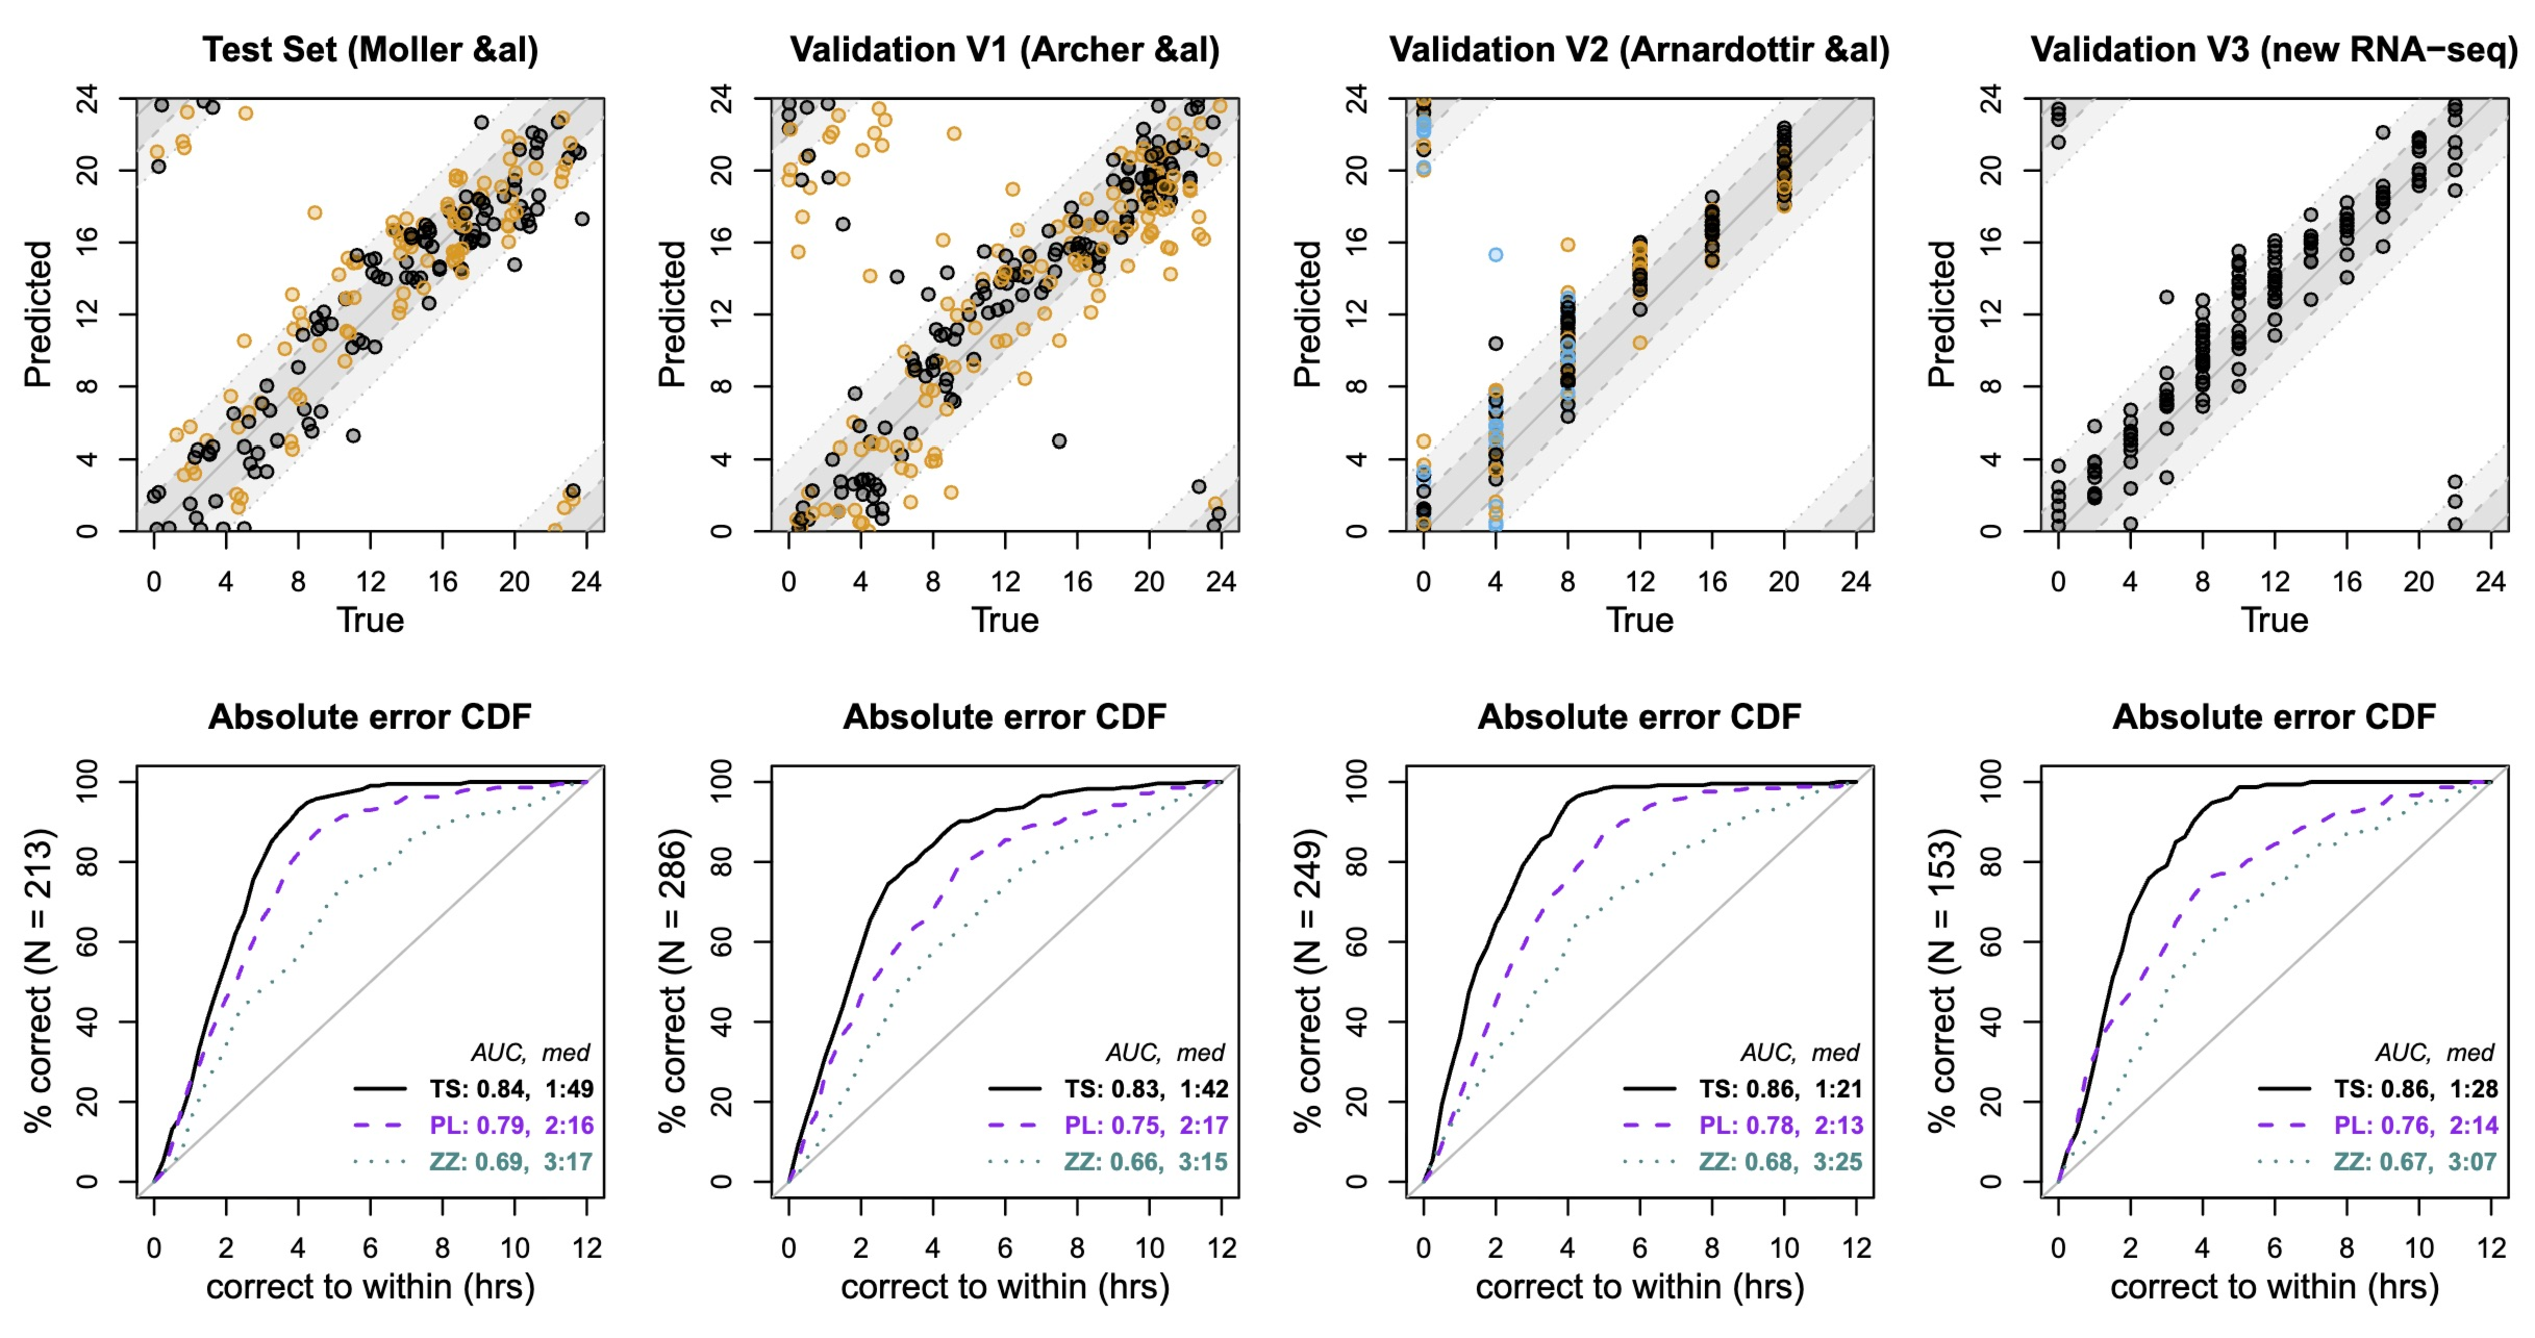
\includegraphics[width=\linewidth]{figure/fig1_original.pdf}
    \caption{Original results reported by Braun et al.\ (2018).}
    \label{fig:fig1_orig}
  \end{subfigure}

  \vspace{6pt}
  \begin{subfigure}{\linewidth}
    \centering
    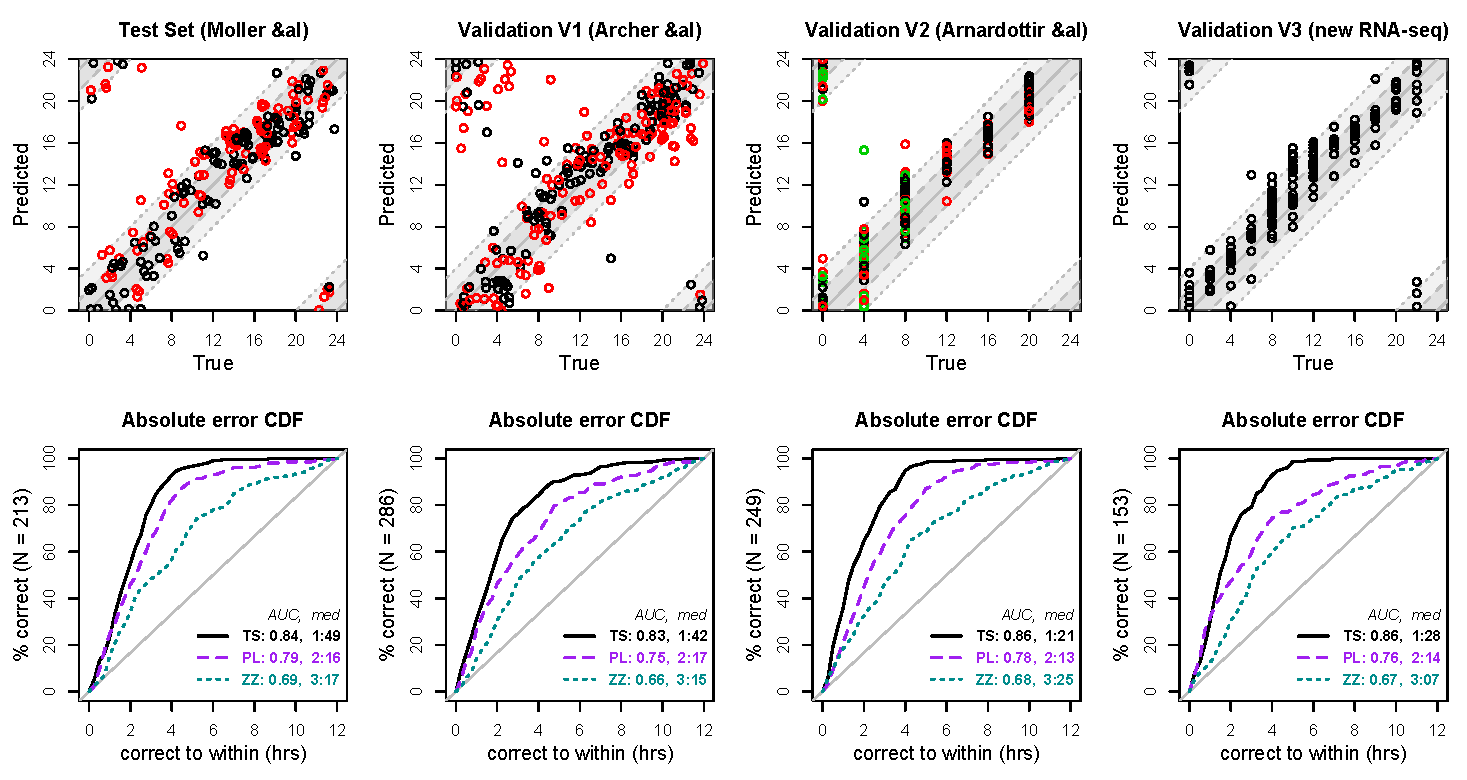
\includegraphics[width=\linewidth]{figure/fig1_reproduced.pdf}
    \caption{Our re-implementation using the full 7,615-gene pool.}
    \label{fig:fig1_repro}
  \end{subfigure}
  \caption{
    \textbf{Reproduction of the TimeSignature cross-study benchmark.}
    Each column corresponds to one of the four datasets of
    Table~\ref{tab:datasets} (test set and validation sets V1--V3),
    and each panel block is arranged in two rows.
    \emph{Top row:} predicted time of day versus true time of day for
    each sample, where the dark and light gray bands indicate error
    ranges of $\pm$2\,h and $\pm$4\,h about the true time;
    point colour denotes experimental condition (in panel (a):
    black, control; orange, sleep restriction or forced desynchrony;
    blue, V2 recovery day), with panel (b) using a distinct colour
    palette to visually separate the two reproductions.
    \emph{Bottom row:} the fraction of correctly predicted samples
    versus the size of the error, shown for three predictors---the
    TimeSignature model (TS, solid black), a PLSR-based model
    (PL, dashed purple), and ZeitZeiger (ZZ, dotted cyan)---with the
    legend listing each method's nAUC and median absolute error.
    \textbf{(a)} The original results reported by Braun et al.\ (2018).
    \textbf{(b)} The same evaluation produced by our re-implementation
    using the full 7,615-gene pool.
    Both reproduce comparable accuracy (nAUC $\geq 0.80$, median
    error $< 2$\,h), confirming that our pipeline reproduces the
    original within-subject-normalization benchmark.
  }
  \label{fig:reproduced_fig1}
\end{figure}

Before extending the model, we verified that our implementation
reproduces the performance reported by Braun et al.\ (2018).
The full 7,615-gene pool (\emph{fullPool}) yielded 172 selected
predictors and achieved nAUC\,${=}\,0.853$ and
MAE\,${=}\,1.89$\,h on the pooled validation set
(Table~\ref{tab:exp2}).
These values match the original Figure~1 benchmark within rounding,
confirming that our pipeline---within-subject normalization, antipodal
calibration, circular elastic net, and nAUC scoring---is correctly
implemented.

\subsection{Experiment 1: JTK\_Cycle Pool Size Sweep}

Experiment~1 asks how far the elastic-net candidate pool can be
reduced---using JTK\_Cycle rhythmicity rank---before accuracy
degrades below the clinical floor.
Figure~\ref{fig:exp1} shows the resulting gene-count versus accuracy
trade-off curve, and Table~\ref{tab:exp1} lists the full sweep of 16
pool sizes.
\begin{figure}[h]
  \centering
  
\includegraphics[width=0.8\textwidth]{figure/Exp1_tradeoff.pdf}
  \caption{
    \textbf{Experiment 1: JTK-filtered pool size versus accuracy.}
    The x-axis (log scale) is the number of top-$K$
    JTK\_Cycle-ranked genes passed to the elastic net.
The left y-axis (navy circles) shows pooled validation nAUC;
    the right y-axis (orange triangles) shows pooled MAE (h).
The red dashed line marks the clinical nAUC floor of 0.80.
All metrics are computed on the three held-out validation
    datasets (V1, V2, V3) combined.
}
  \label{fig:exp1}
\end{figure}

\begin{table}[h]
\centering
\begin{tabular}{rrrrr}
\toprule
Pool $K$ & nSel & MAE (h) & nAUC & \%$\leq$2\,h \\
\midrule
  10  &  10 & 2.40 & 0.810 & 51.0 \\
  15  &  13 & 2.38 & 0.812 & 52.6 \\
  20  &  19 & 2.20 & 0.827 & 58.7 \\
  25  &  23 & 2.21 & 0.826 & 57.6 \\
  30  &  26 & 2.13 & 0.833 & 62.1 \\
  40  &  37 & 2.22 & 0.825 & 57.8 \\
  50  &  42 & 2.11 & 0.834 & 58.9 \\
  75  &  68 & 2.16 & 0.830 & 57.0 \\
 100  &  81 & 2.42 & 0.809 & 53.6 \\
 150  & 102 & 2.42 & 0.809 & 54.9 \\
 200  & 120 & 2.32 & 0.817 & 56.4 \\
 300  & 114 & 2.34 & 0.816 & 53.5 \\
 500  & 151 & 2.48 & 0.803 & 54.4 \\
1000  & 175 & 2.11 & 0.834 & 57.8 \\
2000  & 136 & 1.98 & 0.845 & 60.5 \\
7615  & 173 & 1.89 & 0.853 & 62.2 \\
\bottomrule
\end{tabular}
\caption{Experiment 1 results (pooled validation across V1, V2, V3).
$K$ is the JTK-ranked pool size;
\emph{nSel} is the number of predictors the elastic net
retains from that pool.}
\label{tab:exp1}
\end{table}

The trade-off curve exhibits three notable features.
First, even the smallest pool tested ($K = 10$) clears the
clinical nAUC floor of 0.80 (nAUC\,${=}\,0.810$), demonstrating that
a handful of strongly rhythmic genes contain sufficient circadian
information for clinically useful prediction.
Second, nAUC rises steeply from $K = 10$ to $K = 30$
(nAUC\,${=}\,0.833$, MAE\,${=}\,2.13$\,h) and then plateaus;
increasing the pool from 30 to the full 7,615 genes adds only
$+0.020$ nAUC.
Third, the curve is \emph{non-monotonic} in the intermediate range
($K = 100$--500): nAUC dips to 0.803--0.809, recovering only at
$K \geq 1000$.
This non-monotonicity suggests that moderately ranked genes
(rhythmicity ranks ${\sim}$100--500) introduce noise without
contributing predictive signal, and the elastic net requires a
substantially larger pool before it can reliably separate signal
from noise in this regime.

\subsection{Experiment 2: Published Gene Sets in the TimeSignature
Framework}

Experiment~2 substitutes five published or derived gene sets, plus
the unfiltered full pool, into the same elastic-net pipeline.
Figure~\ref{fig:exp2} presents the pooled validation nAUC for each
set, and Table~\ref{tab:exp2} provides the full performance breakdown.
\begin{figure}[h]
  \centering
  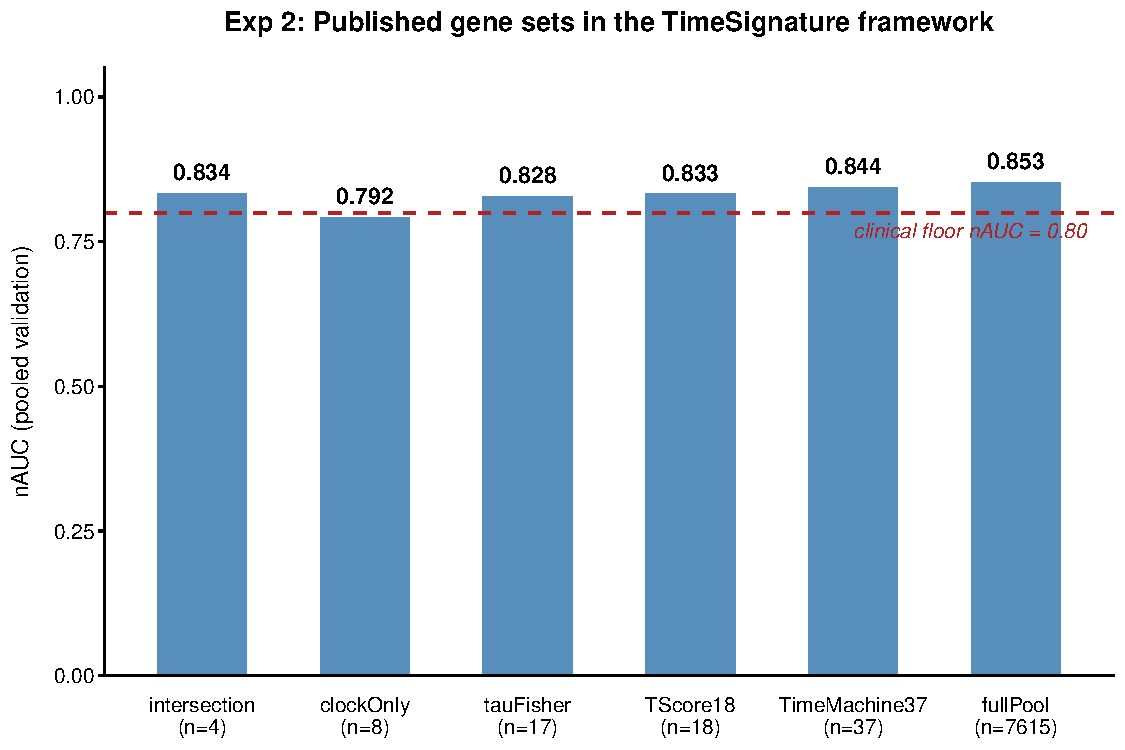
\includegraphics[width=0.8\textwidth]{figure/Exp2_geneset_nAUC.pdf}
  \caption{
    \textbf{Experiment 2: nAUC of published gene sets in the
    TimeSignature framework.}
    Each bar shows the pooled validation nAUC when the elastic net
    is restricted to the indicated gene set.
The red dashed line marks the clinical floor nAUC\,${=}\,0.80$.
    Only clockOnly ($n = 8$) falls below this threshold.
}
  \label{fig:exp2}
\end{figure}

\begin{table}[h]
\centering
\begin{tabular}{llrrrrrr}
\toprule
Gene set & Study & $n_{\mathrm{samp}}$ & nGene & nSel
  & MAE (h) & nAUC & \%$\leq$2\,h \\
\midrule
intersection & V1 & 286 & 4 & 4 & 2.38 & 0.812 & 52.8 \\
             & V2 & 249 & 4 & 4 & 1.80 & 0.860 & 63.1 \\
             & V3 & 153 & 4 & 4 & 2.14 & 0.833 & 58.2 \\
             & \textbf{Valid.all} & \textbf{688} & \textbf{4}
               & \textbf{4} & \textbf{2.12} & \textbf{0.834}
               & \textbf{57.7} \\
\addlinespace
clockOnly    & V1 & 286 & 8 & 8 & 2.87 & 0.771 & 46.9 \\
             & V2 & 249 & 8 & 8 & 2.33 & 0.816 & 55.8 \\
             & V3 & 153 & 8 & 8 & 2.60 & 0.794 & 53.6 \\
             & \textbf{Valid.all} & \textbf{688} & \textbf{8}
               & \textbf{8} & \textbf{2.61} & \textbf{0.792}
               & \textbf{51.6} \\
\addlinespace
tauFisher    & V1 & 286 & 17 & 14 & 2.45 & 0.806 & 51.7 \\
             & V2 & 249 & 17 & 14 & 1.87 & 0.855 & 61.4 \\
             & V3 & 153 & 17 & 14 & 2.22 & 0.825 & 51.6 \\
             & \textbf{Valid.all} & \textbf{688} & \textbf{17}
               & \textbf{14} & \textbf{2.19} & \textbf{0.828}
               & \textbf{55.2} \\
\addlinespace
TScore18     & V1 & 286 & 18 & 18 & 2.27 & 0.822 & 55.2 \\
             & V2 & 249 & 18 & 18 & 1.80 & 0.861 & 65.1 \\
             & V3 & 153 & 18 & 18 & 2.43 & 0.808 & 49.0 \\
             & \textbf{Valid.all} & \textbf{688} & \textbf{18}
               & \textbf{18} & \textbf{2.13} & \textbf{0.833}
               & \textbf{57.4} \\
\addlinespace
TimeMachine37 & V1 & 286 & 37 & 31 & 2.41 & 0.810 & 54.9 \\
              & V2 & 249 & 37 & 31 & 1.70 & 0.869 & 69.9 \\
              & V3 & 153 & 37 & 31 & 1.70 & 0.868 & 66.0 \\
              & \textbf{Valid.all} & \textbf{688} & \textbf{37}
                & \textbf{31} & \textbf{1.99} & \textbf{0.844}
                & \textbf{62.8} \\
\addlinespace
fullPool     & V1 & 286 & 7615 & 172 & 2.07 & 0.838 & 61.2 \\
             & V2 & 249 & 7615 & 172 & 1.69 & 0.869 & 67.9 \\
             & V3 & 153 & 7615 & 172 & 1.88 & 0.854 & 55.6 \\
             & \textbf{Valid.all} & \textbf{688} & \textbf{7615}
               & \textbf{172} & \textbf{1.89} & \textbf{0.853}
               & \textbf{62.4} \\
\bottomrule
\end{tabular}
\caption{Experiment 2 results.  The upper section shows per-study
metrics; the bottom row of each set shows pooled validation
(Valid.all).
Sets are ordered by gene count.}
\label{tab:exp2}
\end{table}

Two key findings emerge from this comparison.
First, the 4-gene intersection (DDIT4, PER1, NR1D1, NR1D2)
achieves nAUC\,${=}\,0.834$, matching the 18-gene TScore18
(nAUC\,${=}\,0.833$) and exceeding the 17-gene tauFisher panel
(nAUC\,${=}\,0.828$).
This result suggests that the majority of the circadian prediction
signal is concentrated in these four genes.
Second, the canonical core-clock panel (clockOnly, $n = 8$) is the
only set falling below the clinical floor (nAUC\,${=}\,0.792$,
MAE\,${=}\,2.61$\,h).
This shortfall demonstrates that the textbook transcriptional
feedback loop is insufficient for accurate circadian-time prediction
in peripheral blood;
rather, data-driven rhythmic genes, selected by
their actual expression amplitude and phase consistency, carry the
signal.
Among all published sets, the reconstructed TimeMachine-37 panel
performs best (nAUC\,${=}\,0.844$, MAE\,${=}\,1.99$\,h), lying within
0.009 nAUC of the full-panel reference.

\subsection{Combined Trade-Off Curve}

Figure~\ref{fig:combined} overlays the Experiment~1 pool-size sweep
with the Experiment~2 gene-set points on a single coordinate system.
This combined view enables direct comparison of each published set
against the JTK-ranked top-$K$ baseline at the same gene count.
\begin{figure}[h]
  \centering
  
\includegraphics[width=0.80\textwidth]{figure/Fig_tradeoff_combined.pdf}
  \caption{
    \textbf{Combined gene-count versus accuracy trade-off.}
    The navy line with filled circles (Experiment~1) shows nAUC as a
    function of JTK-filtered pool size (x-axis, log scale).
Coloured triangles (Experiment~2) mark the pooled validation nAUC
    of five published gene sets overlaid at their respective gene
    counts.
The red dashed line marks the clinical floor nAUC\,${=}\,0.80$.
    Sets falling above the Experiment~1 curve at the same gene count
    achieve higher efficiency than a na\"ive top-$K$ JTK ranking.
  }
  \label{fig:combined}
\end{figure}

The combined figure reveals several additional insights.
The reconstructed TimeMachine-37 panel (nAUC\,${=}\,0.844$) falls
\emph{above} the Experiment~1 curve at $K = 37$
(nAUC\,${=}\,0.825$), indicating that TimeMachine's gene-selection
procedure---core-clock genes prioritized, then JTK-ranked
additions---outperforms a pure top-37 JTK ranking by $+0.019$ nAUC.
The 4-gene intersection likewise sits well above the Experiment~1
curve at its gene count, confirming that these four genes are
disproportionately informative.
In contrast, the clockOnly panel ($n = 8$, nAUC\,${=}\,0.792$) falls
below both the clinical floor and 
the Experiment~1 curve at $K = 10$
(nAUC\,${=}\,0.810$), underscoring that the canonical clock loop
alone is a poor predictor in this framework.

%=====================================================================
\section{Discussion}
%=====================================================================

\subsection{Biological Interpretation}

The results confirm that the circadian prediction signal in human
peripheral blood is concentrated in a small subset of strongly
rhythmic genes rather than distributed across the transcriptome.
The 4-gene intersection achieving nAUC\,${=}\,0.834$ with only DDIT4,
PER1, NR1D1, and NR1D2 is particularly striking.
Two of these genes---NR1D1 (REV-ERB$\alpha$) and NR1D2
(REV-ERB$\beta$)---are core-clock transcriptional repressors with
well-characterized high-amplitude 24-h expression rhythms in
peripheral blood \citep{Reppert2002}.
PER1 is a central period gene whose blood-borne transcript level
peaks in the morning, providing a robust phase marker.
DDIT4 (DNA-damage-inducible transcript 4), a stress-responsive gene,
has been independently identified as a reliable circadian marker in
blood by multiple studies \citep{Braun2018, Huang2024}, suggesting
that its rhythmicity in PBMCs is physiologically meaningful rather
than an artifact of the training cohort.
The failure of the clockOnly set (nAUC\,${=}\,0.792$) is equally
informative.
The eight canonical clock genes present in the assay---including
ARNTL, CRY1, DBP, TEF, and HLF---are expressed at low amplitude
or with high inter-subject variability in blood, limiting their
discriminative power.
This observation is consistent with the broader finding that the
canonical clock network, while necessary for circadian rhythm
generation at the cellular level, does not by itself produce
sufficiently precise markers for population-level circadian
phenotyping from peripheral blood.

\subsection{Non-Monotonicity of the Trade-Off Curve}

An unexpected finding is the non-monotonic dip in nAUC at
intermediate pool sizes ($K = 100$--500), where performance drops
to nAUC\,${=}\,0.803$--0.809 before recovering at $K \geq 1000$
(Table~\ref{tab:exp1}).
One plausible explanation is that genes ranked ${\sim}$100--500 by
JTK\_Cycle have marginal rhythmicity: their expression profiles are
sufficiently periodic to pass the filter but too noisy to contribute
reliable regression signal.
When included in the candidate pool, these genes dilute the
elastic-net penalty budget across many weak predictors, degrading
selection efficiency relative to both the compact ($K \leq 50$) and
very large ($K \geq 1000$) pools.
The full-pool elastic net overcomes this by having enough candidates
for the L1 penalty to identify the sparse informative set even amid
thousands of non-rhythmic features.
This finding suggests that JTK pre-filtering is most beneficial at
\emph{small} pool sizes ($K \leq 50$), where it removes the bulk of
non-rhythmic noise, and that intermediate pre-filtering may actually
harm performance---a counterintuitive result that merits further
investigation.

\subsection{Comparison with Prior Work}

The present work differs from TimeMachine and tauFisher in one key
respect: it retains the original two-blood-draw TimeSignature
framework and asks only whether the \emph{candidate gene pool} should
be pre-filtered, holding the regression architecture, normalization
strategy, and evaluation protocol constant.
This design isolates the effect of gene pre-filtering from
confounding changes in normalization (e.g., TimeMachine's
within-sample ratio features) or model class.
Our Experiment~2 shows that a panel reconstructed by following
TimeMachine's gene-selection procedure achieves nAUC\,${=}\,0.844$
within the two-draw framework, close to the full-pool reference of
0.853.
This proximity suggests that the gene-selection strategy---rather
than the single-sample normalization---accounts for most of the gain
over unfiltered TimeSignature.

\subsection{Practical Implications}

The steep nAUC plateau above $K = 30$ has a direct clinical
implication: a targeted panel of approximately 30 rhythmically ranked
genes suffices for circadian-time estimation under the two-draw
protocol.
This reduction from 7,615 to 30 genes (a 250-fold decrease) would
substantially lower the cost of a dedicated circadian assay relative
to a full microarray, with minimal sacrifice in accuracy
($-0.020$ nAUC, $+0.24$\,h MAE).
The result aligns with the design philosophy of TimeMachine
\citep{Huang2024}, which uses a 37-gene panel and achieves comparable
accuracy, and supports the broader trend towards clinically deployable
circadian clocks.

\subsection{Limitations}

Several limitations should be noted.
First, the JTK\_Cycle ranking is computed on the same GSE39445
training data used to fit the elastic net, introducing a modest
double-dipping risk;
a nested cross-validation design would provide a
more conservative estimate of generalization accuracy.
Second, the training set derives from a controlled sleep-restriction
protocol (${\sim}$213 samples), which makes JTK p-values liberal and
the gene ranking potentially over-fitted to that study population;
ranked lists may differ on community-based or clinically ascertained
cohorts.
Third, the tauFisher and TimeMachine gene sets are reconstructed from
their published procedures using our JTK\_Cycle ranking, rather than
obtained directly from the original authors' exact gene lists, because
the exact symbol lists (e.g., Huang \& Braun 2024 SI Table S2) are
not publicly bundled with the TimeMachine repository.
Fourth, V1 consistently shows lower nAUC than V2 and V3 across all
conditions (Tables~\ref{tab:exp1}--\ref{tab:exp2}), suggesting that
the Archer dataset presents a harder generalization challenge whose
origin (e.g., platform differences, cohort composition) warrants
further investigation.

\subsection{Future Directions}

Two extensions are most promising.
First, applying the same JTK-then-elastic-net pipeline to
single-draw normalization strategies---such as TimeMachine's
within-sample log-ratio features---would test whether pre-filtering
also provides efficiency gains in the more challenging single-sample
setting.
Second, replacing the JTK-based gene selection with a
stability-selection procedure \citep{Meinshausen2010} could yield a
more robust panel that generalises across platforms and training
cohorts.

%=====================================================================
%--- references --------------------------------------------------------
\bibliographystyle{plainnat}
\begin{thebibliography}{99}
\small
\setlength{\itemsep}{0pt}
\setlength{\parskip}{3pt}

\bibitem[Archer et al.(2014)]{Archer2014}
Archer, S.N., Laing, E.E., Möller-Levet, C.S., et al.\ (2014).
Mistimed sleep disrupts circadian regulation of the human
transcriptome.
\emph{PNAS}, \textbf{111}(6), E682--E691.

\bibitem[Antoulas et al.(2018)]{Antoulas2018}
Antoulas, A.C., Zhu, B., Zhang, Q., York, B., O'Malley, B.W.,
\& Dacso, C.C.\ (2018).
A novel mathematical method for disclosing oscillations in gene
transcription: A comparative study.
\emph{PLOS ONE}, \textbf{13}(9), e0198503.

\bibitem[Braun et al.(2018)]{Braun2018}
Braun, R., Kath, W.L., Iwanaszko, M., et al.\ (2018).
Universal method for robust detection of circadian state from gene
expression.
\emph{PNAS}, \textbf{115}(39), E9247--E9256.
\bibitem[Duan \& Ngo(2024)]{Duan2024}
Duan, R.\ \& Ngo, H.\ (2024).
tauFisher predicts circadian time from a single sample of bulk and
single-cell pseudobulk transcriptomic data.
\emph{Nature Communications}, \textbf{15}, 3840.

\bibitem[Huang \& Braun(2024)]{Huang2024}
Huang, P.\ \& Braun, R.\ (2024).
Platform-independent estimation of human physiological time from
single blood samples.
\emph{PNAS}, \textbf{121}, e2308114120.

\bibitem[Hughes et al.(2010)]{Hughes2010}
Hughes, M.E., Hogenesch, J.B., \& Kornacker, K.\ (2010).
JTK\_CYCLE: an efficient nonparametric algorithm for detecting
rhythmic components in genome-scale data sets.
\emph{Journal of Biological Rhythms}, \textbf{25}(5), 372--380.
\bibitem[Meinshausen \& B\"uhlmann(2010)]{Meinshausen2010}
Meinshausen, N.\ \& B\"uhlmann, P.\ (2010).
Stability selection.
\emph{Journal of the Royal Statistical Society: Series B},
\textbf{72}(4), 417--473.
\bibitem[Möller-Levet et al.(2013)]{Moller2013}
Möller-Levet, C.S., Archer, S.N., Bucca, G., et al.\ (2013).
Effects of insufficient sleep on circadian rhythmicity and
expression amplitude of the human blood transcriptome.
\emph{PNAS}, \textbf{110}(12), E1132--E1141.
\bibitem[Reppert \& Weaver(2002)]{Reppert2002}
Reppert, S.M.\ \& Weaver, D.R.\ (2002).
Coordination of circadian timing in mammals.
\emph{Nature}, \textbf{418}, 935--941.

\bibitem[Talamanca et al.(2023)]{Talamanca2023}
Talamanca, L., Gobet, C., \& Naef, F.\ (2023).
Sex-dimorphic and age-dependent organization of 24-hour gene
expression rhythms in humans.
\emph{Science}, \textbf{379}(6631), 478--483.

\bibitem[Ueda et al.(2004)]{Ueda2004}
Ueda, H.R., Chen, W., Minami, Y., et al.\ (2004).
Molecular-timetable methods for detection of body time and rhythm
disorders from single-time-point genome-wide expression profiles.
\emph{PNAS}, \textbf{101}(31), 11227--11232.

\bibitem[Wittenbrink et al.(2018)]{Wittenbrink2018}
Wittenbrink, N., Ananthasubramaniam, B., Münch, M., et al.\ (2018).
High-accuracy determination of internal circadian time from a single
blood sample.
\emph{Journal of Clinical Investigation}, \textbf{128}(9),
3826--3839.


\end{thebibliography}

\end{document}